\chapter{Praktischer Teil}
\label{sec:praktischerteil}
\begin{onehalfspace}
In diesem Teil der Arbeit werden zuerst die beiden Szenarien erläutert und daraufhin die Konzeption und Umsetzung derer in Python beschrieben. Zusätzlich wird die Datenauswertung in Tableaux dargestellt und zum Schluss das Ergebnis der Umsetzung evaluiert.
\section{Szenarien}
\label{subsec:szenarien}
Für das generieren von Daten wurden zwei möglichst reale Szenarien ausgewählt. Zum einen das Szenario eines Bewährungsantrages, für welches 5 verschiedene Attribute und eine endgültige Bewertung mit stattgegeben oder nicht generiert werden. Zum anderen das zweite Szenario des sozialen Punktesystems, für welches pro Person 7 Attribute zu generieren sind und eine numerische Bewertung zwischen 600 und 1400 creditpoints erstellt wird. Diese beiden Szenarien werden im folgenden genauer erläutert.
\subsection{Szenario zur Bewertung von Bewährungsanträge}
\label{subsubsec:szenario1}
In diesem Szenario soll ein Bewährungsantrag einer Person Bewertet werden. Ein aktuelles reales Beispiel dafür stammt aus der USA. In den USA verwenden einige Richter*innen eine Software namens \glqq{}COMPAS\grqq{}, welche eine Vorhersage liefert, wie hoch das Risiko für noch eine weitere Straftat einer Person ist. Die Richter*innen verwenden dies dann um zu entscheiden, ob die Person freigelassen wird oder nicht. Durch eine Untersuchung wurde herausgefunden, dass die Software einen Bias gegenüber Afro-Amerikanischen Menschen besitzt. Dadurch wurden diese in der Entscheidung durch die Software diskriminiert. \cite{Mehrabi2021}\cite{MachineBias2016}\\ 
In diesem für diese Arbeit aufgebauten Szenario besteht ein Antrag dabei aus dem Namen der Person, dessen Geschlecht, Hautfarbe und den entscheidenden Attributen der laufenden Strafe in Jahren und der Härte des Vergehens. Basierend auf diesen Attributen soll eine bewertende Person beurteilen, ob der Antrag genehmigt oder abgelehnt wird. Das Geschlecht wird in \glqq{}Männlich\grqq{} und \glqq{}Weiblich\grqq{} angegeben. Da zur Vereinfachung sich auf das biologische Geschlecht begrenzt wurde und aus diesem Grund die Genderdiversität für den Datengenerator au{\ss}envor gelassen wurde. Die Hautfarbe der Person wird als \glqq{}Schwarz\grqq{} oder \glqq{}Weiß\grqq{} festgehalten. Die noch laufende Strafe des Gefangenen wird als Ganzzahl in Jahren von 1-5 angegeben. Da in diesem Fall ein Bewährungsantrag erst ab maximal 5 Jahren noch offene Strafe gestellt werden. Die Härte des Vergehens wird einfachheitshalber in den Gruppen \glqq{}Leicht\grqq{}, \glqq{}Mittel\grqq{} oder \glqq{}Hart\grqq{} festgehalten. \newline
Für die Beurteilung des Antrags von der bewertenden Person werden folgende Regeln definiert:
\begin{table}[!h]
    \centering
    \begin{tabular}{|l|l|l|}
    \hline
    \textbf{Attribut}   & \textbf{Positive Auswirkung} & \textbf{Negative Auswirkung} \\ \hline
    Laufende Strafe     & 1-3                          & 4-5                          \\ \hline
    Härte des Vergehens & Leicht, Mittel               & Hart                         \\ \hline
    \end{tabular}
\caption{Tabelle für die Auswirkung der Attributen des ersten Szenario}
\label{table:1}
\end{table}\\
Das Geschlecht und die Hautfarbe werden hierbei nicht direkt aufgelistet, da diese in der Regel keine Auswirkung auf die Bewertung haben sollten. Diese können jedoch durch einen konkreten Bias Aussagekraft bekommen. Damit soll in den generierten Daten die gewünschte Verzerrung auf einen gewissen Wert gelegt werden können. In diesem Szenario sind die möglichen Werte, welche durch eine Verzerrung und damit einem menschlichem Vorurteil einer bewertenden Person beeinflusst werden können, das Geschlecht und die Hautfarbe. Die anderen beiden Attribute, welche in der Tabelle \ref*{table:1} aufgeführt sind, wirken sich durch ihre Ausprägungen positiv oder negativ auf die Bewertung des Antrages aus. So wirkt z.B. eine Härte des Vergehens vom Niveau Leicht sich eher für eine positive Bewertung des Antrages aus, als eine mittlere Härte. Dasselbe gilt auch für die Laufende Strafe. So kann eine bewertende Person dann anhand dieser beiden Werte eine Tendenz erhalten und über die Gestattung des Antrages entscheiden.
\subsection{Szenario zur Vorhersage eines sozialen Punktesystems}
\label{subsubsec:szenario2}
Im zweiten Szenario wird das durch China populär gewordene sozial creditpoint system in einer kleineren Version nachgebaut. Dafür werden Einträge zu Personen erstellt, nach welchen die Punktzahl der einzelnen Person zwischen 600 und 1400 Punkten bestimmt wird. Ein Eintrag zu einer Person beinhaltet die sieben in der folgenden Tabelle dargestellten Attribute mit den unterschiedlichen Ausprägungen.
\begin{table}[!h]
    \centering
    \begin{tabular}{|l|l|}
    \hline
    \textbf{Attribut}       & \textbf{Ausprägungen}                                                                                                \\ \hline
    Name                    & Beliebig                                                                                                             \\ \hline
    Alter                   & 20-79                                                                                                                \\ \hline
    Politische Orientierung & Links, Mitte, Rechts                                                                                                 \\ \hline
    Bildungsabschluss       & \begin{tabular}[c]{@{}l@{}}Ausbildung, Fachschulabschluss, \\ Bachelor, Master, Diplom, Promotion, ohne\end{tabular} \\ \hline
    Soziales                & 0-3                                                                                                                  \\ \hline
    Wohnlage                & \begin{tabular}[c]{@{}l@{}}Großstadt, Kleinstadt,\\ Vorort, Ländlich\end{tabular}                                    \\ \hline
    CO2-Fußabdruck          & 4-12                                                                                                                 \\ \hline
    \end{tabular}
\caption{Tabelle der Attribute und Auswirkungen vom Szenario für das soziale Punktesystem}
\label{table:2}
\end{table}
Die in Tabelle \ref*{table:2} aufgeführten Ausprägungen haben ähnlich wie zum Bewährungsantrag Szenario unterschiedlich starke Auswirkungen auf die am Ende bestimmten soziale Punktzahl. Einzig allein der Name und das Alter sollen keine direkte Auswirkung auf die soziale Punktzahl haben. Die anderen Attribute wirken sich je nach Auswirkung positiv durch eine Erhöhung der Punktzahl oder negativ durch eine Verringerung der Punktzahl aus.
Insgesamt werden so in diesem Szenario viele Einträge von Personen erstellt, welche alle unterschiedlichste Verteilungen der Ausprägungen besitzen und dadurch in der Bewertung eine individuelle soziale Punktzahl erzielen. Um nun eine gewünschte Verzerrung in die Daten zu bekommen, können alle Attribute bis auf den Namen, welcher rein als Füllwert dient, durch eine Verzerrung beeinflusst werden. So können z.B. Personen zwischen 20-30 Jahre negativ verzerrt werden, da ein oder zwei Bewertende etwas gegen junge Leute haben und diesen aus ihrer Überzeugung eine schlechtere Punktzahl geben. In diesem Szenario ist somit eine hohe Variabilität geboten inwieweit eine Verzerrung in die Daten gebracht wird. Zudem kann auch eine Verzerrung über mehrere Attribute eingebracht werden, da eine bewertende Person z.B. auch etwas gegen eine Rechte Politische Orientierung und ein schlechtes Soziales Engagement von 0 haben kann.
\subsection{Vergleich der Szenarien}
\label{subsubsec:vergleichSzenarien}
Ein Überblick über beiden Szenarien ist in der nachfolgenden Tabelle \ref{table:vergleichSzenarien} dargestellt. 
\begin{table}[!h]
    \begin{tabular}{|c|c|c|c|c|}
    \hline
    \textbf{Szenario}    & \textbf{Attribute} & \textbf{Zusammenhänge} & \textbf{Bias} & \textbf{Bewertung}                                                  \\ \hline
    Bewährungsanträge    & 5                         & 2                      & Lable Bias    & \begin{tabular}[c]{@{}c@{}}genehmigt\\ nicht genehmigt\end{tabular} \\ \hline
    Soziale Punktesystem & 7                         & 5                      & Lable Bias    & \begin{tabular}[c]{@{}l@{}}Punkte von:\\ 600 bis 1400\end{tabular}  \\ \hline
    \end{tabular}
    \caption{Tabelle für den Vergleich beider Szenarien}
\label{table:vergleichSzenarien}
\end{table}\\
In der Tabelle werden die Szenarien auf deren Anzahl an Attributen, die Zusammenhänge, die zu generierende Art des Bias und die Art der Bewertung eines Datenpunktes verglichen. In der Anzahl der Attribute und damit auch den Zusammenhängen unterscheiden sich die Szenarien stark. Das Szenario der Bewährungsanträge besitzt nur 5 Attribute und dadurch nur 2 Zusammenhänge zwischen diesen. Beim sozialen Punktesystem sind es schon 7 Attribute und daher auch 5 Zusammenhänge in diesen, wodurch dieses Szenario insgesamt deutlich komplexer wird. Da zum einen mehr Daten pro Datenpunkt generiert werden und die größere Anzahl an Zusammenhängen einen höheren Interpertationsspielraum bieten. Die Art des Bias ist bei beiden Szenarien gleich, da wir betrachten wie sich die Vorurteile von Menschen beim bewerten/\glqq{}labeln\grqq{} von Personen aufs maschinelle Lernen auswirken. Daher wird hier beides Mal der unter \ref{subsubsec:Bias} beschrieben Label Bias generiert. Die Bewertung, welche den Bias dann beinhaltet, ist in beiden Szenarien unterschiedlich. Im ersten Szenario der Bewährungsanträge wird binär in genehmigt oder nicht genehmigt bewertet. Beim sozialen Punktesystem hingegen wird eine Punktzahl als Ganzzahl zwischen 600 bis 1400 angegeben, dadurch steigert sich die Komplexität dieses Szenario erneut.\\
Insgesamt sind die Szenarien damit bis auf die Art des Bias vor allem in der Komplexität deutlich unterschiedlich gestaltet. Dadurch ergibt sich ein etwas leichteres erstes Szenario der Bewährungsanträge und ein komplexeres mit mehr Freiraum gestaltetes Szenario zur Vorhersage eines sozialen Punktesystems.
\section{Konzeption}
\label{subsection:konzeption}
In diesem Kapitel wird die erarbeitete Konzeption für die Umsetzung der beiden im Kapitel \ref*{subsec:szenarien} aufgeführten Szenarien erläutert. Dabei wird in ein Grobkonzept zur allgemeinen Generierung der Daten und daraufhin ein Feinkonzept für jedes Szenario unterteilt.
\subsection{Grobkonzept}
\label{subsubsec:grobkonzept}
Das Grobkonzept beinhaltet die Überlegungen, wie die Programme/Notebooks für die beiden Szenarien generell aufgebaut sein sollen. Der Ablauf der Programme von der Eingabe der Parameter bis hin zu den fertig generierten Daten wird in fünf Schritten durchgeführt. Der Ablauf der Schritte ist in folgendem Programmablaufplan dargestellt.\\
\begin{figure}[h]
    \centering
    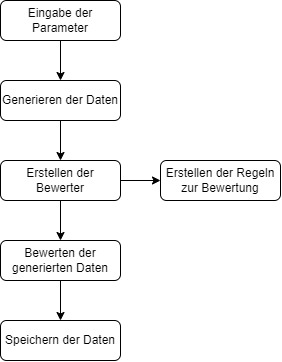
\includegraphics[width=6cm,height=8cm]{Diagramme/Grobkonzept_PAP.jpg}
    \caption{Programmablaufplan der fünf Hauptschritte zur Generierung der Daten}
    \label{fig:GrobkonzeptPAP}
\end{figure}\\
Die in der Abbildung \ref{fig:GrobkonzeptPAP} dargestellten Hauptschritte des Programmablaufs lauten: Parametereingabe, Generieren der Daten, Regeln aufstellen, Bewerten und Speichern der Daten. Im ersten Schritt der Parametereingabe, wird den Benutzenden die Möglichkeit gegeben die Parameter für die Generierung der Daten einzugeben, wie z.B. die Anzahl der Daten oder Bewertende welche generiert werden sollen. Im folge Schritt wird die passende Anzahl an Daten für das jeweilige Szenario generiert. Dabei sollen die Daten möglichst an Verhältnissen aus der Realität angepasst und auf dieser Grundlage generiert werden. Es soll jedoch eine gewisse Zufälligkeit in der Generierung vorhanden sein, sodass bei mehrfach Generierung unterschiedliche Datensätze auf Basis der definierten Verteilungen entstehen. Nach Abschluss der Generierung wird der fertige Datensatz zwischengespeichert, um diesen später bewerten zu können. Für die Bewertung des Datensatzes muss im folgenden 3. Schritt die Regeln nach welchen bewertet wird aufgestellt werden. Dafür soll zuerst die in den Parametern gewünschte Anzahl an Bewertenden erstellt werden, da durch diese die Regeln erstellt werden. Unter den erstellten Bewertenden müssen zudem noch die angegebene Anzahl an diskriminierenden Bewertenden in solche umgewandelt werden. Daraufhin können dann die Regeln für die Bewertenden erzeugt werden. Somit ist der 3. Schritt abgeschlossen und alle Vorbereitungen getroffen für die Bewertung. In der Bewertung bekommen die Bewertenden alle Anträge des Datensatzes vorgelegt, welche Sie basierend auf den Regeln bewerten. Die Bewertung des jeweiligen Antrages wird diesem in den Daten hinzugefügt. Damit kann zum letzten Prozess übergegangen werden. In diesem wird der Ursprungsdatensatz und der bewertete Datensatz abgespeichert und damit auch au{\ss}erhalb von dem Programm zugänglich gemacht.\\
Somit ist das Grobkonzept der Szenarien abgeschlossen und ein Grundgerüst konnte entworfen werden. Im weiteren kann nun auf die detaillierte Feinkonzeption der einzelnen Szenarien eingegangen werden.
\subsection{Feinkonzept}
\label{subsubsec:feinkonzept}
Die im Grobkonzept beschriebenen fünf Hauptschritte der Programme sind für beide Szenarien gleich. Jedoch unterscheiden sich die Schritte im Detail bei beiden Szenarien. Daher wird für jedes Szenario ein eigenes Feinkonzept zur Füllung des selben vorhanden Grundgerüst entwickelt.\\
\textbf{Parametereingabe}\\
Im ersten Schritt der Parametereingabe unterscheiden sich die Szenarien nicht, da beide einen Parameter für die gewünschte Diskriminierung, die Anzahl der Daten, die Anzahl der Bewertenden, die Anzahl der diskriminierenden Bewertenden und der stärke der Auswirkung von der Diskriminierung benötigen. Diese Parameter können von den Benutzenden in beiden Fällen in einer finalen Zelle editiert werden.\\
\textbf{Daten generieren}\\
In diesem Prozess unterscheiden sich beide Szenarien stark, da zum einen für das erste Szenario nur fünf anstelle von sieben Attribute generiert werden müssen und zum anderen existieren deutlich weniger Verbindungen zwischen den Attributen im ersten Szenario anstelle vom zweiten. Bei den Bewährungsanträgen basiert, wie in Abbildung \ref{fig:VerbindungenS1} dargestellt, nur die Härte der Strafe und die Hautfarbe auf dem Geschlecht, dies bedeutet die Wahrscheinlichkeiten für diese Attribute sollen dem Geschlecht entsprechend angepasst werden.
\begin{figure}[h]
    \centering
    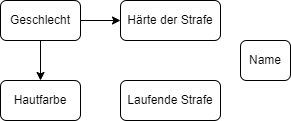
\includegraphics{Diagramme/Verbindung_der_Attribute_S1.drawio.png}
    \caption{Verbindungen zwischen den Attributen eines Bewährungsantrages}
    \label{fig:VerbindungenS1}
\end{figure}\\
So haben zum Beispiel weibliche Personen eher seltener eine Harte Strafe als männliche Personen. Die beiden anderen Attribute in diesem Szenario haben, wie in der Abbildung \ref{fig:VerbindungenS1} gezeigt, keine Verbindung und daher eine feste Wahrscheinlichkeitsverteilung. Damit sind die Zusammenhänge in diesem Szenario sehr klein gehalten und überschaubar.\\
Im Szenario des sozialen Punktesystems müssen sieben Attribute generiert werden und es sollen deutlich mehr Verbindungen zwischen diesen existieren. Um diese verständlich darzustellen wurde ein Diagramm für das Feinkonzept entworfen, welches nachfolgend dargestellt ist.\\
\begin{figure}[h]
    \centering
    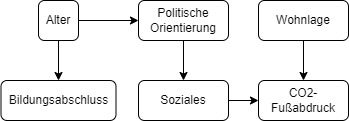
\includegraphics{Diagramme/Verbindung_der_Attribute_S2.jpg}
    \caption{Verbindungen zwischen den Attributen des zweiten Szenario}
    \label{fig:VerbindungenS2}
\end{figure}\\
In der Abbildung \ref{fig:VerbindungenS2} sind alle Attribute, bis auf das Attribut Name, des zweiten Szenario als abgerundete Rechtecke und die Verbindungen zwischen diesen mit Pfeilen dargestellt. Insgesamt existieren fünf Verbindungen zwischen den Attributen. Diese sollen so aufgebaut werden, um möglichst Realitätsnahe Daten generieren zu können. Die Verbindung zwischen dem Alter und dem Bildungsabschluss existiert, da zum Beispiel die Wahrscheinlichkeit, dass eine Person mit 20 schon eine Promotion besitzt nicht so hoch ist wie bei einer Person im Alter von 50. Zudem hat das Alter einen Einfluss auf die Politische Orientierung einer Person, da junge Leute sicherlich andere Orientierungen haben als Personen im Alter von 50 zum Beispiel, siehe Aktionen wie \glqq{}FridaysforFuture\grqq{}. Durch die Politische Orientierung einer Person wird in diesem Fall auch mit einer Beeinflussung auf das soziale Verhalten gerechnet und es besteht daher hier auch eine Verbindung. Im Falle des CO2-Fußabdruck wird in dieser Arbeit mit einer Auswirkung der Wohnlage und des Sozialen gerechnet. Durch das Soziale und die Vorverbindungen wird die Politische Orientierung und das Alter ebenfalls indirekt darauf mit ein bezogen. Dies ist hier der Fall, da die Berechnung des CO2-Fußabdruck sich aus vielen Faktoren zusammensetzt und daher auch dieser in diesem Szenario durch viel beeinflusst werden soll. Durch diese Zusammenhänge sollen dann möglichst realitätsnahe Daten entstehen.\\
Insgesamt müssen für beide Szenarien später bei der Umsetzung die Wahrscheinlichkeiten der Ausprägungen der Attribute, wo es möglich ist, durch Statistiken bestimmt und die Verbindungen dadurch ebenfalls bestätigt werden. Dies wird im Kapitel \ref{umsetzung} im Detail erläutert.\\
\textbf{Regeln aufstellen}\\
Im diesem Schritt werden zuerst bei beiden Szenarien die gewünschte Anzahl an Bewertenden erstellt, von welchen danach die Anzahl an diskriminierenden ausgewählt wird. In der Folge können die Regeln für die zuvor als Objekte erstellte Bewertenden erstellt werden. Im Fall des ersten Szenarios werden zwei Listen mit Hilfe der unter Kapitel \ref{subsubsec:szenario1} gezeigten Tabelle erstellt. Eine Liste beinhaltet die in der Tabelle dargestellten positiven Auswirkungen und die andere Liste beinhaltet die negativen Auswirkungen. So haben die Objekte der Bewertenden ihre eigenen Listen an Regeln. Daher kann für die diskriminierenden Bewertenden in der Liste der negativen Auswirkungen das zu diskriminierende Attribut hinzugefügt werden. So diskriminieren diese Bewertenden automatisch, da sie diese Regeln zur Überprüfung der Bewertung haben. Für das zweite Szenario sieht das Konzept hier etwas anders aus, da es hier nicht um eine Bewertung in genehmigt oder nicht geht, sondern um Punkte. Somit müssen die Regeln so erstellt werden, dass die Bewertenden eine Liste an allen Ausprägungen der Attributen haben und dazu eine passende Zuordnung mit wie vielen Punkten sich welche Ausprägung auf die Punktzahl auswirkt. Die Verzerrung wird in diesem Fall erst im nächsten Schritt der Bewertung betrachtet.\\
\textbf{Bewertung}\\
Folgend auf die erstellten Regeln können die Bewertenden nun die vorgelegten Einträge der Daten bewerten. Im ersten Szenario wird das ganze durch eine Wahrscheinlichkeitsverteilung durchgeführt. Zu Beginn jeder Bewertung steht es 50:50 für genehmigt oder nicht. Durch die erstellten Regel-Listen können dann die Bewertenden die im Antrag aufgeführten Attribute abgleichen, ob diese sich positiv (also für eine Genehmigung) oder negativ auswirken. Nach dieser Bestimmung wird dann die Wahrscheinlichkeitsverteilung verschoben in positive oder negative Richtung. So kann am Ende wenn der Bewertende alle Attribute durch hat, mit Hilfe der übrig gebliebenen Wahrscheinlichkeiten für positiv und negativ eine Entscheidung getroffen werden. Falls ein bewertendes Objekt diskriminierend sein sollte, hat dieses wie oben erläutert in seinen negativen Regeln die gewünschte Ausprägung enthalten, sodass diese sich dann auf die Entscheidung auswirkt. Für das zweite Szenario wird nicht mit einer Wahrscheinlichkeitsverteilung gearbeitet, sondern mit dem mittleren Wert der Punktzahl als Startwert(1000). So können die Bewertenden von Attribut zu Attribut aus dem zu bewertenden Eintrag durchlaufen und entsprechend nach der Ausprägung den in Ihren eigenen Regeln definierte Wert dem Startwert hinzu addieren. Damit entsteht dann letztendlich die finale Punktzahl für den Eintrag. Für die Verzerrung wird das Attribut und die Ausprägung dessen welche verzerrt werden soll in jedem Eintrag gesucht. Falls die gewünschte Ausprägung vorhanden ist, wird die Punktzahl dieses Eintrages um die in den Parametern eingegebene negative Auswirkung für die Verzerrung addiert.\\
Insgesamt werden bei beiden Szenarien die Einträge aus dem generierten Datensatz zufällig einem Bewertenden zur Bewertung zugeordnet. So ist eine zusätzliche Variabilität in der Verteilungen der Verzerrung gegeben.\\
\textbf{Speichern der Daten}\\
Zum Abschluss werden bei beiden Szenarien gleich, die beiden Datensätze als CSV Datei gespeichert. Zum einen den ursprünglich generierten Datensatz und zum anderen auch der Datensatz mit der jeweiligen Bewertung enthalten. Durch eine CSV Datei können die Daten dann beliebig in anderen Programmen weiterverwendet werden.\\ \\
Insgesamt ist damit die Konzeption abgeschlossen. Im Grobkonzept wurde ein Grundgerüst für die beiden Programme der Szenarien entworfen, welches auch für noch weitere Szenarien der Art verwendet werden kann. Im Feinkonzept wurde dann das Grundgerüst durch Inhalt der jeweiligen Szenarien gefüllt und das geplante im Detail beschrieben. So kann nun zur Umsetzung der beiden Programme übergegangen werden. 

\section{Umsetzung}
\label{umsetzung}
In diesem Kapitel wird die konkrete Umsetzung der beiden Szenarien in einzelnen Unterkapiteln beschrieben.
\subsection{Umsetzung des Szenario zur Bewertung von Bewährungsanträge}
\label{umsetzungsz1}
Da die Programme als sogenannte Notebook Dateien in Python umgesetzt sind, können die einzelnen, in der Konzeption dargestellten, Prozessschritte als Zellen verwirklicht werden. Das Python Notebook stammt von Jupyter und ist ein open source Projekt für eine interaktive Codeplatform, auf welcher neben Code auch Visualisierungen und Text eingebracht werden können. Die Dateien heißen dann Notebooks und enden mit \glqq{}.ipynb\grqq{}. Nun wird die Umsetzung des ersten Szenarios beschrieben.\\
Im Programm für das erste Szenario, welches \glqq{}Szenario1.ipynb\grqq{} heißt, müssen in der ersten Zelle die benötigten Bibliotheken geladen werden.
Die Bibliothek \glqq{}numpy\grqq{} wird für Zufallsauswahlen unter bestimmten Wahrscheinlichkeiten benötigt. \glqq{}faker\grqq{} ist eine Bibliothek für generierte Daten, so wird diese hier für das bestimmen zufälliger Namen verwendet. \glqq{}pandas\grqq{} bietet sogenannte Dataframes, in welchen die Daten gespeichert werden und durch \glqq{}pandas\grqq{} auch in eine CSV Datei geschrieben werden können. Die letzte Bibliothek \glqq{}random\grqq{} ist ebenfalls wie \glqq{}numpy\grqq{} für das generieren von Zufallswerten zuständig. Zum Schluss wird in der Zelle noch eine Instanz der Faker Klasse erstellt, welche zur Verwendung der Bibliothek benötigt wird.\\
In der nächsten Zelle ist die Methode \glqq{}create\_fake\_data\grqq{} zur Generierung der Daten umgesetzt. Diese Methode bekommt die beiden Parameter \glqq{}num\grqq{} und \glqq{}seed\grqq{} übergeben. Der Parameter \glqq{}seed\grqq{} wird zu Beginn verwendet um den Startwert der Faker Instanz und von \glqq{}numpy\grqq{} zu setzen. Dadurch wird es ermöglicht, mit unterschiedlichen Startwerten, eine nahezu \glqq{}echte\grqq{} Zufallszahl zu generieren. Bei gleichbleibendem Startwert und gleicher Methode würde der Code immer die gleiche Zufallszahlen bestimmen. Zum Beispiel wenn drei Zahlen von 0-10 generiert werden sollen, werden bei gleichem Startwert immer die drei selben Zahlen generiert. Variiert der Startwert jedoch, werden jedes Mal unterschiedliche Zahlen generiert und eine ausreichende Variabilität erreicht. Als nächstes wird mit einer Schleife über die im Parameter \glqq{}num\grqq{} angegebene Zahl iteriert. In jedem Schleifendurchlauf wird ein Eintrag für den Datensatz generiert. Somit ist \glqq{}num\grqq{} die Größe des gewünschten Datensatzes. In diesem Szenario müssen somit in jedem Durchlauf ein Wert für die Attribute Name, Geschlecht, Härte der Strafe, Hautfarbe und Laufende Strafe ermittelt werden. Der Name in jedem Eintrag wird durch die Faker Instanz generiert. Dafür wird je nach Geschlecht die Methode zum generieren eines weiblichen oder männlichen Namen aufgerufen. Die Attribute Geschlecht, Härte der Strafe und Hautfarbe müssen nach bestimmten Wahrscheinlichkeiten berechnet werden. Dies wird für jedes dieser Attribute wie folgend ausgeführt:\\
\textbf{Geschlecht}\\
Formel zur Berechnung der Wahrscheinlichkeiten für \ac{M} und \ac{W}:\\
Gegeben: Gesamt = Gesamt Zahl der Gefangenen\\
\begin{equation}
    W/M\% = \frac{W/M}{Gesamt}\label{eq:Sz1Mänlich}
\end{equation}
\begin{table}[!h]
    \centering
    \begin{tabular}{|c|c|c|}
    \hline
    \textbf{Ausprägungen} & \textbf{Berechnung} & \textbf{Wahrscheinlichkeit} \\ \hline
    Weiblich              &\rule{0pt}{18pt} $\frac{105.000}{1.439.800}$  & 7,3\% \\[8pt] \hline
    Männlich              & \rule{0pt}{18pt}$\frac{1.334.800}{1.439.800}$     & 92,7\%  \\[8pt] \hline
    \end{tabular}
\caption{Tabelle zur Bestimmung der Wahrscheinlichkeiten für das Geschlecht}
\label{table:3}
\end{table}\\
Das Geschlecht für eine Person wird nach den in der Tabelle \ref{table:3} berechneten Wahrscheinlichkeiten bestimmt. Die hier berechneten Wahrscheinlichkeiten ergeben sich aus den Gefängniszahlen von 2017 der USA, welche in einem Beitrag des U.S. Department of Justice im April 2019 veröffentlicht wurden. Die Zahlen wurden hierbei aus der \glqq{}Table 8\grqq{} des Papers entnommen und zur Berechnung nach der oben aufgeführten Formel verwendet.\cite[S. 17]{Bronson2017}\\
Die daraus entstehenden Wahrscheinlichkeiten werden wie in dem folgenden Listing \ref{lst:GeschlechtscodeS1} zur Bestimmung des Geschlechts mit Hilfe der \glqq{}numpy\grqq{} Bibliothek verwendet.\\
\begin{lstlisting}[language=Python,label={lst:GeschlechtscodeS1},caption=Codezeile zur Bestimmung des Geschlechts einer Person nach angegebenen Wahrscheinlichkeiten]
sex = np.random.choice(["M", "W"], p=[0.927, 0.073])
\end{lstlisting}
In der Zeile Code werden zuerst die möglichen Ausprägungen als Strings in einem Array angegeben und dann die dazugehörigen Wahrscheinlichkeiten nach welchen eine Ausprägung bestimmt werden soll.\\
\textbf{Härte der Strafe}\\
Für die Bestimmung einer Ausprägung der Härte der Strafe, ist die Berechnung der Wahrscheinlichkeiten und die letztendliche Auswahl etwas komplexer. Da wie in der Konzeption geplant die Härte der Strafe vom Geschlecht einer Person abhängig ist. Daher ist es nicht möglich eine einfache Formel zur Berechnung aufzustellen, sondern es muss aus der Datenquelle erörtert werden wie sich die Wahrscheinlichkeiten verteilen. Die Verteilung der Wahrscheinlichkeiten ist in der folgenden Tabelle dargestellt.\\
\begin{table}[h]
    \centering
    \begin{tabular}{|l|l|l|}
    \hline
    \textbf{Ausprägungen} & \textbf{Weiblich} & \textbf{Männlich} \\ \hline
    Leicht                & 36,1\%            & 26,6\%            \\ \hline
    Mittel                & 26,4\%            & 16,9\%            \\ \hline
    Hart                  & 37,5\%            & 56,5\%            \\ \hline
    \end{tabular}
\caption{Tabelle der Wahrscheinlichkeiten für die Härte der Strafe nach Geschlecht}
\label{table:4}
\end{table}\\
Die in Tabelle \ref{table:4} gezeigten Wahrscheinlichkeiten ergeben sich aus dem Beitrag des U.S. Department of Justice vom April 2019. In diesem ist in \glqq{}Table 12\grqq{} eine prozentuale Verteilung von den Strafgruppen Gewalttätig, Eigentum, Drogen, Öffentliche Ordnung und Sonstige über die Geschlechter \ac{W} und \ac{M} aus dem Dezember 2016 aufgelistet. Dabei sind die Strafen nach den schwersten Delikten absteigend aufgeführt. Somit wird diese Verteilung auf die in der Konzeption definierten Ausprägungen Leicht, Mittel und Hart verteilt. So wird der Prozentsatz der gewalttätigen Strafen Hart zugeordnet, die Eigentumsstrafen Mittel zugeordnet und die Drogen, Öffentliche Ordnung und Sonstigen Strafen Leicht zugeordnet. Dadurch ergeben sich auf Grundlage der Zahlen aus den USA die Wahrscheinlichkeiten in der Tabelle \ref{table:4}.\cite[S. 21]{Bronson2017}\\
Um die Bestimmung der Härte der Strafe nun durchzuführen, wird der selbe Code wie im Listing \ref{lst:GeschlechtscodeS1} gezeigt auf dieses Attribut angepasst und im Verbund mit einer if Abfrage zur Überprüfung des Geschlechts umgesetzt. So wird entsprechend dem Geschlecht einer Person nach den dazu passenden Wahrscheinlichkeiten die Härte der Strafe zufällig ausgewählt.\\
\textbf{Hautfarbe}\\
Formel zur Berechnung der Hautfarbe basierend auf dem Vorwissen des Geschlechtes:\\
Gegeben: Gesamt \ac{W}/\ac{M} = Anzahl an Weißen und Schwarzen Gefangenen pro (G)Geschlecht = S(Schwarz) + Wi(Weiß)\\
\begin{equation}
    S/Wi\% = \frac{S/Wi}{Gesamt \ac{W}/\ac{M}}\label{eq:Sz1Hautfarbe}
\end{equation}
\begin{table}[h]
    \centering
    \begin{tabular}{|c|c|c|}
    \hline
    \textbf{Ausprägungen} & \textbf{Berechnung} & \textbf{Wahrscheinlichkeit} \\ \hline
    Schwarz              &\rule{0pt}{28pt} $
        S\%= 
    \begin{cases}
        \frac{456.300}{843.700}\quad |&\text{Geschlecht: M}\\
        \frac{19.600}{68.700} \quad | &\text{Geschlecht: W}
    \end{cases}$ & \(\displaystyle S\%=
    \begin{cases}
    54,1\%\quad | & \text{Geschlecht: M} \\
    28,5\%\quad| & \text{Geschlecht: W}
    \end{cases} \) \\[22pt] \hline
    Weiß              &\rule{0pt}{28pt} $
        Wi\%= 
    \begin{cases}
        \frac{387.400}{843.700}\quad |& \text{Geschlecht: M}\\
        \frac{49.100}{68.700} \quad |&\text{Geschlecht: W}
    \end{cases}$ & \(\displaystyle Wi\%=
    \begin{cases}
    45,9\%\quad | & \text{Geschlecht: M} \\
    71,5\%\quad | & \text{Geschlecht: W}
    \end{cases} \) \\[22pt] \hline
    \end{tabular}
\caption{Tabelle zur Bestimmung der Wahrscheinlichkeiten für die Hautfarbe unter Berücksichtigung des Geschlechts}
\label{table:5}
\end{table}\\
Die in der Tabelle \ref{table:5} dargestellten Berechnungen und daraus resultierenden Wahrscheinlichkeiten beruhen erneut auf der Veröffentlichung vom U.S. Department of Justice. In dieser sind in \glqq{}Table 8\grqq{} die Gefangenen nach Geschlecht und ethischen Gruppen aufgeteilt. Zur Vereinfachung wurden für die Hautfarbe jedoch nur zwischen Schwarz und Weiß unterschieden. Dabei werden Ethnien bewusst nicht gesondert berücksichtigt. Somit sind lediglich die Zahlen für die Anzahl an der Gruppe Schwarz und Weiß nach Geschlecht Männlich Weiblich von Interesse. Um daraus Prozentwerte zu bilden, nach welchen dann eine Person entweder die Hautfarbe Schwarz oder Weiß bekommt, wurde die oben gezeigte Formel aufgestellt. Für die Formel wird zuerst zum einen die Gesamtheit an Schwarzen sowie Weißen männlichen Personen und zum anderen die Gesamtheit an Schwarzen sowie Weißen weiblichen Personen gebildet. Daraufhin können basierend auf diesen Gesamtwerten die Wahrscheinlichkeitsverteilungen für Männlich und Schwarz, Männlich und Weiß, Weiblich und Schwarz, Weiblich und Weiß anhand der Formel berechnet werden.\\
Damit diese Wahrscheinlichkeiten bei der Bestimmung angewendet werden können, wird wie schon bei der Härte der Strafe, der Code aus Listing \ref{lst:GeschlechtscodeS1} durch eine if Abfrage erweitert und an dieses Attribut angepasst.\\
Als letztes Attribut wird noch eine Ausprägung für die Länge der Strafe bestimmt. Hierfür wird mit der \glqq{}numpy\grqq{} Bibliothek eine zufällige Ganzzahl zwischen eins und fünf ausgewählt.\\
Um einen Schleifendurchlauf abzuschließen werden die durch Wahrscheinlichkeiten bestimmten Werte zusammen als ein Dictionary als neuen Eintrag in ein Array mit der Zuordnung(Attribut:Ausprägung) hinzugefügt. Damit ist ein Schleifendurchlauf abgeschlossen und der nächste kann beginnen. Wenn die Schleife fertig ist, wird das volle Array mit den gespeicherten Einträgen aus der Methode, zum Datengenerieren, zurückgegeben und diese ist damit auch vollends durchgeführt.\\
Als nächsten, aus der Konzeption definierten Prozessschritt, nach dem generieren der Daten, wird das aufstellen der Regeln umgesetzt. Hierfür wird die Methode \glqq{}create\_Rules\grqq{} mit den Parametern \glqq{}request\_values, request\_bias, bias\grqq{} implementiert. Der Parameter \glqq{}request\_values\grqq{} ist ein Dictionary mit den Keys an den für die Bewertung relevanten Attributen und den dazugehörigen Ausprägungen in einem Array als Value. In diesem Fall sind es wie in der Konzeption definiert die Attribute Härte der Strafe und Laufende Strafe, welche wie in der folgenden Abbildung \ref{lst:RequestValues} im Dictionary angegeben werden.\\
\begin{lstlisting}[language=Python,label={lst:RequestValues},caption=Codezeilen zum Erstellen eines Dictionary mit den zur Bewertung relevanten Attributen]
request_values = {
    "Laufende_Strafe": [1,2,3,4,5],
    "Haerte_des_Vergehens": ["Leicht", "Mittel", "Hart"]
}
\end{lstlisting}
Der Parameter \glqq{}request\_bias\grqq{} ist genau gleich aufgebaut, beinhaltet jedoch die Attribute Geschlecht und Hautfarbe und deren Ausprägung. Dieser gibt die Liste der durch Verzerrung beeinflussbaren Attribute an. Der letzte Parameter \glqq{}bias\grqq{} gibt die gewünschte Verzerrung ebenfalls wie die anderen Parameter an. 
In der Methode werden vier Rückgabewerte als Dictionaries generiert. Ein Dictionary für die Regeln der positiven Auswirkung, eines für die negative Auswirkung und nochmals die selben zwei Listen ergänzt durch die gewünschte Verzerrung. 
\begin{figure}[h]
    \centering
    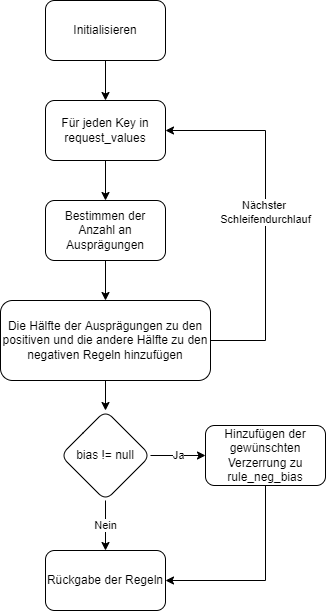
\includegraphics[width=8cm,height=14cm]{Diagramme/Sz1_Regeln.drawio.png}
    \caption{Programmablaufplan zur Generierung der Regeln vom Szenario für Bewährungsanträge}
    \label{fig:Sz1Regeln}
\end{figure}\\
In Abbildung \ref{fig:Sz1Regeln} ist der Ablauf der Methode als Programmablaufplan skizziert. Zu Beginn werden die vier Dictionaries, in welchen die Regeln gespeichert werden, initialisiert. Daraufhin wird eine Schleife durch alle Keys des \glqq{}request\_values\grqq{} Dictionary durchlaufen. Darin werden als erstes die Anzahl an Ausprägungen des in diesem Durchlauf ausgewählten Attributes gezählt. Nach dem die Anzahl an Ausprägungen klar ist, kann die Mitte bestimmt werden. Anhand der Mitte werden die Ausprägungen unterhalb und gleich der Mitte dem Dictionary der negativen Regeln hinzugefügt und die restlichen oberhalb der Mitte dem Dictionary der positiven Regeln. Wenn dies vollbracht ist, ist der erste Durchlauf beendet und es kann mit dem nächsten weiter gemacht werden. Solange bis alle \glqq{}request\_values\grqq{} den Regeln zugeordnet sind. Danach werden die erstellten Dictionaries für die positiven und negativen Regeln in die Dictionaries für die Bias Regeln kopiert.
Im nächsten Punkt wird überprüft, ob ein Bias angegeben wurde. Wenn kein Bias angegeben wurde, werden die zuvor erstellten und kopierten Regeln als die vier Dictionaries zurückgegeben. Falls ein Bias angegeben wurde, wird für jeden Key in \glqq{}request\_bias\grqq{} überprüft, ob dieser dem angegebenen Attribut entspricht. Sobald der Key und damit das Attribut, welches verzerrt werden soll, gefunden ist werden die Ausprägungen, welche im Bias angegeben wurden, den negativen Bias Regeln hinzugefügt und die anderen übrig gebliebenen den positiven Bias Regeln hinzugefügt. So wird zum Beispiel bei Angabe: \glqq{}bias: Hautfarbe:Weiß\grqq{} die Hautfarbe:Weiß den negativen Bias Regeln und die Hautfarbe:Schwarz den positiven Bias Regeln hinzugefügt. Daraufhin sind alle vier Dictionaries für die Regeln gefüllt und können zurückgegeben werden.
Damit ist die Methode zum erstellen der Regeln vollständig umgesetzt.
In der nächsten Zelle wurde eine Methode zum generieren eines Seeds/Startwerts umgesetzt. Dieser wird wie zu Beginn der Umsetzung beschrieben benötigt, um zu jedem Ausführungszeitpunkt unterschiedliche Zufallswerte zu erhalten. Daher sollte der Startwert ebenfalls immer variieren. Um dies zu schaffen werden momentane Zeitwerte genommen und miteinander verrechnet, sodass am Ende ein zeitabhängiger Wert resultiert. Zur Absicherung, falls der Wert Mal negativ oder Null sein sollte, wird ein zweiter alternativ Wert aus dem aktuellen Tag multipliziert mit den aktuellen Minuten plus Eins berechnet, da bei dieser Rechnung immer ein Wert größer Null resultiert. Der am Ende berechnete Startwert wird dann zurückgegeben und kann somit verwendet werden.    
Im nächsten Prozessschritt wird wie in der Konzeption beschrieben, das Erstellen der Bewertenden und die Methode zum Bewerten umgesetzt. Dafür wird eine Klasse namens \glqq{}Evaluator\grqq{} erstellt, welche die Methoden \glqq{}init\grqq{} und \glqq{}rate\grqq{} implementiert. Der Aufbau der Methode \glqq{}init\grqq{} ist in dem folgenden Listing \ref{lst:Evaluator_init} dargestellt.
\begin{lstlisting}[language=Python,label={lst:Evaluator_init},caption=Methode zur Initialisierung eines Bewertenden]
def __init__(self, rule_pos, rule_neg, bias, percentage=0.2):
    self.rule_pos = rule_pos
    self.rule_neg = rule_neg
    self.bias = bias
    self.bias_percentage = percentage
\end{lstlisting}
Die Methode ist für das Erstellen eines Objektes mit den angegebenen Parametern zuständig. Dabei wird jedem \glqq{}Evaluator\grqq{} Objekt ein Dictionary mit positiven Regeln und eines mit negativen Regeln sowie ein Boolean ob der Bewertende diskriminierend ist und ein Prozentsatz, welcher die stärke der Diskriminierung angibt, übergeben. Diese vier Angaben speichert jedes Objekt für sich und kann intern für sich selbst darauf zugreifen. Damit können dann die gewünschte Anzahl an Bewertenden und Bewertende welche diskriminieren erstellt werden. Durch die Angaben der eigenen Regeln, haben dann die diskriminierenden Bewertenden die Bias Regeln und die neutralen Bewertenden die normalen Regeln. Zudem kann durch das Flag als Boolean ein diskriminierender von einem neutralen Bewerter unterschieden werden.
Die zweite Methode der Klasse, welche \glqq{}Evaluator\grqq{} implementiert und von jedem Objekt der Klasse verwendet werden kann, ist in dem folgenden Listing \ref{lst:Evaluator_rate} dargestellt.
\begin{lstlisting}[language=Python,label={lst:Evaluator_rate},caption=Methode eines Bewertenden zum Bewerten von Anträgen]
def rate(self, request, bias):
    #First 50/50 distribution
    pos = 50
    #Calculate the proportion according to which the decision is influenced positively or negatively.
    prop = 45/self.rule_pos.__len__()
    #Depending on how the rules match the request, the weight of the positive evaluation is shifted.
    for key in self.rule_pos.keys():
        if(self.rule_pos[key].__contains__(request[key])):
            pos += prop
        else:
            pos -= prop
    try:
        #If a bias is present, this is additionally taken into account with the Parameter in %
        if(self.bias):
            for b in bias:
                if(bias[b].__contains__(request[b])):
                    pos = pos*self.bias_percentage
        #Normalise positive value
        pos = pos/100
        #Determine negative value
        neg = 1-pos
        #Rating by chance with indication of pos and neg rating and adding the rating to the request. 
        request["Bewertung"] = np.random.choice(["positiv", "negativ"], p=[pos, neg])
    except:
        print("Failure")
    return request
\end{lstlisting}
Die hier gezeigte Methode \glqq{}rate\grqq{} wird von den Objekten der Klasse \glqq{}Evaluator\grqq{} zum Bewerten eines Antrages verwendet. Als Parameter werden zum einen mit \glqq{}self\grqq{} das Objekt welches die Methode aufruft, mit \glqq{}request\grqq{} der zu bewertende Antrag und mit \glqq{}bias\grqq{} die Verzerrung welche ausgewirkt werden soll übergeben. Als Rückgabe wird der erhaltene Antrag mit Ergänzung der Bewertung zurückgegeben. Im Nachfolgenden wird erläutert wie die Bewertung in der Methode abläuft.
Zu Beginn wird die Wahrscheinlichkeitsverteilung zwischen der positiven und negativen Bewertung auf 50 zu 50 Prozent gesetzt. Somit ist die Entscheidung noch offen. Danach wird eine Proportion bestimmt, durch welche sich eine im Antrag positive oder negative Ausprägung auf die Wahrscheinlichkeitsverteilung der Entscheidung auswirkt. Diese wird wie folgt errechnet: 45 geteilt durch die Anzahl an Attributen in den Regeln. Es wird mit 45 gerechnet, da es immer noch eine rest Wahrscheinlichkeit geben soll, falls alle Ausprägungen im Antrag positiv oder negativ ausfallen. Als nächstes werden die Ausprägungen der Attribute im Antrag durch eine Schleife mit den Regeln verglichen, um aus den Regeln zu entscheiden, ob die Wahrscheinlichkeitsverteilung der Entscheidung die Proportion hinzu oder abgezogen wird. So tendiert die Entscheidung am Ende mehr zu einer positiven oder negativen Entscheidung abhängig von den im Antrag angegebenen Ausprägungen und den Regeln des Bewertenden. Um nach der Bewertung noch eine potentielle Diskriminierung einzubringen, wird überprüft ob das Flag des Bewertenden zur Diskriminierung gesetzt ist. Wenn die Bewertende Person eine diskriminierende und die gewünschte Bias Ausprägung in dem Antrag vorhanden ist, wird die Wahrscheinlichkeit für eine positive Auswirkung durch die Code Zeile: \glqq{}pos = pos*self.bias\_percentage\grqq{} mit dem für den Bewertenden angegebenen Prozentsatz verringert. Somit ist dadurch die Möglichkeit auf eine positive Bewertung deutlich gesunken. Nachfolgend wird dann noch die Wahrscheinlichkeitsverteilung für die Entscheidung passend umgewandelt, um beruhend auf diesen Wahrscheinlichkeiten die Entscheidung zu treffen und das Ergebnis im Antrag also dem Dataframe anzuhängen. Zum Schluss wird der überarbeitete Antrag wieder zurückgegeben und das Bewerten ist abgeschlossen.\\
Nach Abschluss der Klasse werden nun noch zwei Methoden benötigt, welche den gesamt Ablauf durchführen und die anderen Methoden vereinen. Zum einen die Methode \glqq{}generate\_data\grqq{}, welche die Anzahl an zu generierenden Datensätzen übermittelt bekommt. In der Methode wird zuerst ein Seed durch Aufruf der oben beschriebenen Methode zum Seed/Startwert generieren erzeugt. Danach kann die Methode für das Datengenerieren mit dem Seed und der Anzahl an Daten aufgerufen werden. Der Rückgabewert wird dann in ein neuen Pandas Dataframe geschrieben und zurückgegeben. Die andere Methode, welche implementiert wird, ist für den gesamt Ablauf der Datenbewertung zuständig. Diese trägt den Namen \glqq{}work\grqq{} und bekommt den Datensatz, die gewünschte Verzerrung, die Anzahl der Bewertenden, die Anzahl der diskriminierenden Bewertenden und die Prozentual Auswirkung der Verzerrung als Parameter übergeben. Als erstes werden in der Methode die beiden benötigten Dictionaries für \glqq{}request\_values und request\_bias\grqq{} angelegt und mit den Werten des Szenarios nach dem Schema wie in dem obigen Listing \ref{lst:RequestValues} zu sehen gefüllt. Danach werden daraus die Regeln bestimmt und gespeichert. Im Anschluss wird die gewünschte Anzahl an \glqq{}Evaluator\grqq{} Objekte erzeugt und diesen die Regeln übergeben. Um die Verzerrung umzusetzen wird danach die gewünschte Anzahl der \glqq{}Evaluator\grqq{} Objekte in diskriminierende Bewertende umgewandelt und dessen Regeln ausgetauscht durch die Bias Regeln. Damit sind alle Vorbereitungen abgeschlossen und das eigentliche Bewerten der Anträge kann beginnen. Dafür wird eine Schleife über den Dataframe der Anträge durchlaufen. Für jeden Antrag wird dann zufällig bestimmt, welches \glqq{}Evaluator\grqq{} Objekt den Antrag bewertet. Nachdem der Antrag bewertet wurde wird dieser der Liste der fertigen Anträge hinzugefügt. Sobald alle Anträge bewertet sind und die Schleife daher durchlaufen ist, wird die Liste der fertigen Anträge zu einem Dataframe umgewandelt und aus der Methode zurückgegeben. 
Damit sind auch die letzten beiden Methoden umgesetzt und es muss letztendlich nur noch eine finale Zelle zur Ausführung des gesamten Programmes erstellt werden.\\
\begin{lstlisting}[language=Python,label={lst:Sz1finalCell},caption=Letzte Zelle des Szenario der Bewährungsantrag für die Interaktion des Benutzenden]
#Here is the section for the possible parameters to enter
#This dictionary specifies the bias(es) on a possible attribute
bias = {
    "Hautfarbe": ["Schwarz"]
}
#The number of datasets that are to be generated
datasets=10000
#The number of evaluators who evaluate entries
evaluator_count=10
#The number of evaluators who evaluate with a bias
bias_evaluator=4
#This decides how strong the bias will be. The higher the stronger.
bias_percentage=0.2

#Dont touch this
data = generate_data(datasets)
finished = work(data,bias,evaluator_count,bias_evaluator,bias_percentage)
data.to_csv("Daten.csv", sep=';', encoding='utf-8', index=False)
finished.to_csv("Daten_Bewertet.csv", sep=';', encoding='utf-8', index=False)
\end{lstlisting}
Im Listing \ref{lst:Sz1finalCell} ist die letzte Zelle für die Interaktionen des Benutzenden dargestellt. Im oberen Teil der Zelle haben die Benutzenden die Möglichkeit, Anpassungen am Datengenerator zu machen. So kann hier die gewünschte Verzerrung, die Größe des Datensatzes, die Anzahl an Bewertenden, die Anzahl der diskriminierenden unter den Bewertenden und der Prozentuale Einfluss der Verzerrung angepasst werden. Im unteren Teil wird dann die Hauptmethode zum Datengenerieren (generate\_data) aufgerufen und im Anschluss durch die Methode \glqq{}work\grqq{} die zuvor generierten Anträge bewertet. Beide Datensätze werden separat als Variablen geführt, sodass am Ende der Methode die Ursprungsdaten als \glqq{}Daten.csv\grqq{} und der bewertete Datensatz als \glqq{}Daten\_Bewertet.csv\grqq{} abgespeichert werden.\\
Insgesamt ist mit dieser letzten Zelle die gesamte Umsetzung des ersten Szenarios als \glqq{}Szenario1.ipynb\grqq{} Datei abgeschlossen und kann so direkt verwendet werden, um Daten zu generieren.
\subsection{Umsetzung des Szenario zur Vorhersage von einem sozialen Punktesystem}
\label{umsetzungsz2}
Das zweite Szenario wird ebenfalls wie das erste in eine Python Notebook umgesetzt. Das File trägt den Namen \glqq{}Szenario2.ipynb\grqq{} und beginnt sowie auch das erste Szenario mit dem laden der benötigten Bibliotheken. Auch in diesem werden die gleichen Bibliotheken obig zum ersten Szenario beschrieben geladen. Einzige Ausnahme hierbei liegt darin, dass das Faker Objekt nicht wie in der Abbildung gezeigt ist erstellt wird. In diesem Fall wir es wie folgt erstellt: \glqq{}fake = Factory.create("de\_DE")\grqq{}. Der Grund dafür, liegt darin, dass in diesem Szenario Deutsche Namen generiert werden sollen, da es sich um ein auf Deutschland angelegtes Szenario handelt. In der zweiten Zelle des Notebooks wird die Methode für das erstellen eines Seed/Startwert aus dem Szenario der Bewährungsanträge implementiert. Diese verändert sich nicht und kann daher so verwendet werden.\\
Als nächstes ist die Methode \glqq{}create\_fake\_data\grqq{} mit den Parameter num und seed umgesetzt. In dieser wird die durch num angegebene Anzahl an Daten generiert. Der Parameter seed wird zu beginn der Methode als Startwert für die Zufallsmethoden von numpy und Faker gesetzt. Als nächstes wird eine Schleife über num begonnen, in welcher in jedem Durchlauf einen Eintrag für den Datensatz generiert wird. In jedem Durchlauf müssen die Ausprägungen der für dieses Szenario bestimmte Attribute Name, Alter, Politische Orientierung, Bildungsabschluss, Soziales, Wohnlage und CO2-Fußabdruck, unter Betrachtung der im Kapitel \ref{subsection:konzeption} angegebenen Abhängigkeiten, bestimmt werden. Der Name eines Eintrages wird durch die Faker Instanz wie folgt \glqq{}"Name": fake.first\_name()\grqq{} generiert. Die anderen Ausprägungen der Attribute werden, um das Szenario so real wie möglich zu halten, beruhend auf Wahrscheinlichkeiten aus Statistiken bestimmt. Die Wahrscheinlichkeiten der verschiedenen Attributen ergeben sich wie folgend aufgeführt:\\
\textbf{Alter}\\
Ein Alter für eine Person wird zwischen 20 und 79 Jahren bestimmt. Zur Bestimmung wird aufgrund der verwendeten Statistik in drei Altersgruppen unterteilt, welche unterschiedliche Wahrscheinlichkeiten besitzen. Die Altersgruppen sind von 20 bis 39, 40-59 und 60 bis 79 Jahren.\\
Die Formel zur Berechnung der Wahrscheinlichkeiten:\\
Gegeben: Gesamt(Personen im Alter zwischen 20-79) = 20,36 + 23,38 + 18,15 = 61,89 Millionen\\
\begin{equation}
    Altersgruppe\% = \frac{Altersgruppe}{Gesamt}\label{eq:Sz2Alter}
\end{equation}
\begin{table}[!h]
    \centering
    \begin{tabular}{|c|c|c|}
    \hline
    \textbf{Altersgruppen} & \textbf{Berechnung} & \textbf{Wahrscheinlichkeit} \\ \hline
    20-39                  & \rule{0pt}{18pt} $\frac{20,36}{61,89}$ & 33\%   \\[8pt] \hline
    40-59                  & \rule{0pt}{18pt} $\frac{23,38}{61,89}$ & 38\%  \\[8pt] \hline
    60-79                  & \rule{0pt}{18pt} $\frac{18,15}{61,89}$ & 29\%   \\[8pt] \hline
    \end{tabular}
    \caption{Tabelle zur Bestimmung der Wahrscheinlichkeiten für die Altersgruppen}
    \label{table:6}
\end{table}\\
Die in der Tabelle \ref{table:6} nach der Formel \ref{eq:Sz2Alter} errechneten Wahrscheinlichkeiten beruhen auf der Statistik des Statistischen Bundesamt vom 31. Dezember 2020.\cite{statista2020} Die Zahlen wurden passend zu den Altersgruppen aus der Statistik entnommen. Um nun aus den errechneten Wahrscheinlichkeiten auf ein Alter zu kommen, wird im Code zu erst die Altersgruppe nach den Wahrscheinlichkeiten bestimmt. Nachdem die Altersgruppe klar ist, wird eine Zufallszahl im Bereich der Altersgruppe bestimmt, welche dann das endgültige Alter ist. Dadurch wird eine gute Verteilung des Alters entsprechend der Statistik gewährleistet.\\
\textbf{Politische Orientierung}\\
Bei der Bestimmung der Politischen Orientierung in Links, Mitte und Rechts wird wie in der Abbildung \ref{fig:VerbindungenS2} aus Kapitel \ref{subsubsec:feinkonzept} dargestellt, dass Alter als Grundlage mit verwendet. Daher ist die Berechnung und damit auch die Wahrscheinlichkeitsverteilung pro Altersgruppe für die Politische Orientierung unterschiedlich. Des weiteren wird, um die Daten so realitätsnahe wie möglich zu halten, eine statistische Auswertung des Wahlverhaltens bei der Bundestagswahl 2017 nach Alter hinzugezogen. Da in der Statistik die Ergebnisse in Prozent pro Partei angegeben sind, wurde nach eigenem Ermessen entscheiden, welche Partei zu welcher Ausprägung zugeordnet wird. Zur Ausprägung Mitte gehört dabei die CDU, SPD, CSU und FDP zu Links Die Linke und Grüne und zu Rechts wird die AFD zugeordnet. Daraus lassen sich dann die in der folgenden Tabelle \ref{table:7} aufgelisteten Wahrscheinlichkeiten nach dem Alter berechnen.\cite[S. 33]{konrad-adenauer-stiftung2021}\\
\begin{table}[!h]
    \centering
    \begin{tabular}{|c|c|c|c|c|c|c|}
    \hline
    \textbf{Ausprägungen} & \textbf{20-24} & \textbf{25-34} & \textbf{35-44} & \textbf{45-59} & \textbf{60-69} & \textbf{70-79} \\ \hline
    Links                 & 28,0\%         & 24,4\%         & 21,6\%         & 20,7\%         & 17,7\%         & 10,7\%         \\ \hline
    Mitte                 & 63,1\%         & 61,4\%         & 61,8\%         & 63,5\%         & 68,7\%         & 80,9\%         \\ \hline
    Rechts                & 8,9\%          & 14,2\%         & 16,6\%         & 15,8\%         & 13,6\%         & 8,4\%          \\ \hline
    \end{tabular}
    \caption{Tabelle der Wahrscheinlichkeiten für die Politische Orientierung nach Alter}
    \label{table:7}
\end{table}\\
Die in der Tabelle \ref{table:7} dargestellten Wahrscheinlichkeiten wurden nach den dafür angegebenen Altersgruppen aus der Tabelle der Veröffentlichung von der Konrad-Adenauer-Stiftung e. V. berechnet. Dafür wurden die Prozente der oben zugeordneten Parteien aufsummiert. So ergeben sich die Prozentpunkte für Links, Mitte und Rechts. Jedoch fehlen zu den 100\% pro Altersgruppe die Prozentpunkte der Sonstigen Parteien. Da diese nämlich keiner Richtung zugeordnet werden können müssen die Prozente der sonstigen Insgesamt verrechnet werden. Nach der Verrechnung der Sonstigen Parteien entstehen dann die in der Tabelle dargestellten Wahrscheinlichkeiten.\cite[S. 33]{konrad-adenauer-stiftung2021} Zur Umsetzung der Bestimmung der Politischen Orientierung wird eine Reihe an ifelse Abfragen über das zutreffende Alter durchlaufen, um dann mit den Altersendsprechenden Wahrscheinlichkeiten die Politische Orientierung zu bestimmen. Der Code für die Wahrscheinlichkeitsauswahl sieht dabei genau wie im Beispiel aus dem Listing \ref{lst:GeschlechtscodeS1} dargestellt aus.\\
\textbf{Bildungsabschluss}\\
Der Bildungsabschluss einer Person basiert ebenfalls wie die Politische Orientierung auf dem Alter. Zusätzlich wird wie auch schon zuvor eine Statistik aus einem Datenreport des Jahres 2021 vom Statistischen Bundesamt verwendet. \cite{destatis2021} Dadurch können die Daten so realitätsnahe wie möglich gehalten werden.\\ 
\begin{table}[!h]
    \centering
    \begin{tabular}{|c|c|c|c|c|c|}
    \hline
    \textbf{Ausprägungen} & \textbf{\textless{}=29} & \textbf{30-39} & \textbf{40-49} & \textbf{50-59} & \textbf{\textgreater{}=60} \\ \hline
    Ausbildung            & 42,5\%                  & 45,2\%         & 51,6\%         & 55,9\%         & 54,4\%                     \\ \hline
    Fachschulabschluss    & 8,1\%                   & 9,1\%          & 9,7\%          & 11,3\%         & 9,6\%                      \\ \hline
    Bachelor              & 11,7\%                  & 5,9\%          & 1,4\%          & 0,5\%          & 0,2\%                      \\ \hline
    Master                & 7,1\%                   & 5,2\%          & 1,1\%          & 0,3\%          & 0,1\%                      \\ \hline
    Diplom                & 5,9\%                   & 15,7\%         & 17,9\%         & 15,9\%         & 13,2\%                     \\ \hline
    Promotion             & 0,3\%                   & 1,6\%          & 1,7\%          & 1,4\%          & 1,2\%                      \\ \hline
    Ohne                  & 24,4\%                  & 17,3\%         & 16,6\%         & 14,7\%         & 21,3\%                     \\ \hline
    \end{tabular}
    \caption{Tabelle der Wahrscheinlichkeiten für den Bildungsabschluss nach Alter}
    \label{table:8}
\end{table}\\
Die in der Tabelle \ref{table:8} dargestellten Wahrscheinlichkeiten für die dort aufgeführten Altersgruppen ergeben sich aus der \glqq{}Tab 9\grqq{} des Datenreports vom Statistischen Bundesamt. Die Daten der \glqq{}Tab 9\grqq{} stammen aus dem Jahr 2018 der deutschen Bevölkerung. Für die Altersgruppe von 20 bis 29 Jahre existiert keine passende Angabe in der Quelle, da in dieser erst ab dem Alter von 25 Jahren Werte aufgelistet sind. Einfachheitshalber wird daher für die Personen kleiner gleich 29 Jahre die Werte der Personen zwischen 25 und 29 Jahren genommen. Dasselbe gilt auch für die Personen älter als 60, hier werden in der Quelle nur eine Wertereihe für Personen mit 60 und älter angegeben. Das Szenario bezieht sich jedoch nur bis 79 Jahre und passt somit hier auch nicht vollkommen. Zur Vereinfachung wird hierbei jedoch diese Wertereihe für alle zwischen 60 und 79 Jahren verwendet.\cite{destatis2021}\\
\textbf{Soziales}\\
Das soziale Engagement wird von 0 bis 3 angegeben und basiert wie in der Konzeption beschrieben, um die Daten interessanter zu machen, auf der Politischen Orientierung. Durch solche Abhängigkeiten gestalten sich die Daten nämlich realitätsnaher und bringen eine größere Variabilität mit. Da jedoch für die Werte keine Referenzen aus der realen Welt zur Verfügung stehen, wird mit fiktiven Werten gearbeitet.\\
\begin{table}[!h]
    \centering
    \begin{tabular}{|c|c|c|c|}
    \hline
    \textbf{Ausprägungen} & \textbf{Links} & \textbf{Mitte} & \textbf{Rechts} \\ \hline
    0                     & 40\%           & 60\%           & 75\%            \\ \hline
    1                     & 25\%           & 20\%           & 15\%            \\ \hline
    2                     & 25\%           & 15\%           & 9\%             \\ \hline
    3                     & 10\%           & 5\%            & 1\%             \\ \hline
    \end{tabular}
    \caption{Tabelle der Wahrscheinlichkeiten für das Soziale Engagement nach Politischer Orientierung}
    \label{table:9}
\end{table}\\
Die in der Tabelle \ref{table:9} aufgeführten fiktiven Wahrscheinlichkeiten sind ebenso wie schon bei der Bestimmung der anderen Attribute, durch den Code aus Listing \ref{lst:GeschlechtscodeS1} umgesetzt. Jedoch wird durch eine if else Abfrage die unterschiedlichen Politischen Orientierungen unterschieden und dementsprechend die passenden Wahrscheinlichkeiten in der Codezeile verwendet.\\
\textbf{Wohnlage}\\
Die Wohnlage wird durch die Ausprägungen Ländlich, Vorort, Kleinstadt und Großstadt angegebenen und wird durch kein anderes Attribut beeinflusst. Die Wahrscheinlichkeiten für die einzelnen Ausprägungen sind in nachfolgender Tabelle aufgezeigt.
\begin{table}[!h]
    \centering
    \begin{tabular}{|c|c|c|}
    \hline
    \textbf{Ausprägungen} & \textbf{Einwohnergrenze} & \textbf{Wahrscheinlichkeit} \\ \hline
    Ländlich              & \textless{}= 2000        & 5,38\%                      \\ \hline
    Vorort                & 2.000 - 5000             & 8,5\%                       \\ \hline
    Kleinstadt            & 5.000 - 20.000           & 26,6\%                      \\ \hline
    Großstadt             & \textgreater 20.000      & 59,52\%                     \\ \hline
    \end{tabular}
    \caption{Tabelle der Wahrscheinlichkeiten für die Wohnlage}
    \label{table:10}
\end{table}\\
Zur Bestimmung der Wahrscheinlichkeiten für die unterschiedlichen Ausprägungen der Wohnlage müssen zuerst die in der Tabelle \ref{table:10} angegebenen Einwohnergrenzen pro Ausprägung festgelegt werden. Für die Festlegung wurde nach eigenem Ermessen entschieden, welche Ausprägung zu welcher Einwohnergrenze passt. Aus einer Publikation des Statistischen Bundesamt können dann nach dieser Eingliederung die Wahrscheinlichkeiten aufsummiert werden. In der Publikation \glqq{}Gemeinden nach Bundesländern und Einwohnergrößenklassen am 31.12.2020\grqq{} sind der prozentuale Anteil an deutschen Einwohner in gewissen Einwohnergrenzen angegeben. Diese werden dann nach den hier für die Ausprägungen definierten Grenzen aufsummiert und in der Tabelle angegebenen. Damit kann eine möglichst Realitätsnahe Datenerzeugung gewährleistet werden. Für die Umsetzung der Auswahl der Ausprägung kann wie auch schon in den vorigen Fällen der selbe Code aus Listing \ref{lst:GeschlechtscodeS1} auf den Fall hier angepasst und verwendet werden. So sieht die finale Codezeile wie in der folgenden Abbildung dargestellt aus.
\begin{lstlisting}[language=Python,label={lst:Sz2AuswahlWohnlage},caption=Codezeile zur Auswahl der Ausprägung der Wohnlage basierend auf angegebenen Wahrscheinlichkeiten]
location = np.random.choice(["Großstadt","Kleinstadt","Vorort","Ländlich"], p=[0.5952,0.266,0.085,0.0538])
\end{lstlisting}
\textbf{CO2-Fußabdruck}\\
Der CO2-Fußabdruck ist das komplexeste Attribut des Szenarios, da dieser auf zwei Attributen basiert. Wie in der Abbildung \ref{fig:VerbindungenS2} dargestellt hat das Soziale Engagement und die Wohnlage eine Auswirkung auf den CO2-Fußabdruck. Dadurch, dass das Soziale Engagement ebenfalls noch von der Politischen Orientierung und diese vom Alter abhängig ist, haben auch noch zwei weitere Attribute eine indirekte Auswirkung auf den CO2-Fußabdruck. Dies lässt sich auch dadurch begründen, dass der CO2-Fußabdruck in der Realität sich aus vielen unterschiedlichen Teilen zusammensetzt. Da es für den CO2-Fußabdruck unter Berücksichtigung dieser Auswirkungen keine Referenzen aus der realen Welt gibt, wurden fiktive Werte für eine Gaußkurve verwendet. Als Referenzen für die Angabe der Ausprägung des CO2-Fußabdruck in Tonnen pro Kopf konnte jedoch der Mittelwert von 7,91 Tonnen herangezogen werden.\cite{ClimateWatch2022} Um daraus ein Intervall um diesen Wert als Mittelwert festzulegen. So ergab sich das Intervall von 4 bis 12 Tonnen in 0,5er Schritten. Für die daraus resultierenden 17 Ausprägungen wurde eine Gaußkurve erzeugt. Um die Auswirkung von Sozialem Engagement und Wohnlage durchzusetzen wird die Gaußkurve, je nach Grundlage der Attribute verschoben. Für die Umsetzung der jeweiligen Verschiebung durch die beiden Attribute Soziales Engagement und Wohnlage muss eine große ifelse Abfragestruktur mit 16 unterschiedlichen Zuständen erstellt werden, da beide Attribute 4 verschiedene Ausprägungen haben(4*4=16). In den 16 unterschiedlichen Zuständen wird dann die Codezeile aus dem Listing \ref{lst:Sz2AuswahlWohnlage}, um die 17 Ausprägungen des CO2-Fußabdruck angepasst und die Wahrscheinlichkeiten der Gaußkurve entsprechend dem Zustand eingetragen. Dadurch entsteht ein recht komplexes Codekonstrukt, welches jedoch sehr anschauliche abhängige Daten liefert und damit das Szenario in der Auswertung interessanter gestaltet.\\
Mit der abschließenden Bestimmung des CO2-Fußabdruck sind alle Ausprägungen der Attribute bestimmt und die Werte können nun als ein Dictionary dem Array des gesamt Datensatzes hinzugefügt werden.
\begin{lstlisting}[language=Python,label={lst:Sz2AddEntry},caption=Codeausschnitt zum Hinzufügen eines Dateneintrags zum gesamt Datenset]
output.append(
    {
        #Name of the person
        "Name": fake.first_name(),
        "Alter": age,
        "Politische Orientierung": politics,
        "Bildungsabschluss": grad,
        "Soziales": social,
        "Wohnlage": location,
        "CO2-Fußabdruck": co2
    }  
)
\end{lstlisting}
Im Listing \ref{lst:Sz2AddEntry} ist der Codeausschnitt zu sehen, wie das Dictionary mit der Zuordnung Attribut als Key und die Ausprägung als Value erstellt und dem Array \glqq{}output\grqq{} angehängt wird. Die Ausprägung des Namens wird in diesem Schritt erst bestimmt und die anderen werden durch die Variablen übertragen.
Im Anschluss ist ein Schleifendurchlauf beendet, somit ein Eintrag dem Datensatz hinzugefügt und es wird falls noch offen der nächste Durchlauf begonnen. Sobald die Schleife beendet ist, ist der gesamte gewünschte Datensatz generiert und wird letztendlich nur noch als Array aus der Methode zurückgegeben. \\
Als nächste Zelle wird wie auch schon im ersten Szenario eine Methode, welche das Datenerstellen zusammenfasst umgesetzt. Diese ist genau gleich wie im Kapitel \ref{umsetzungsz1} beschrieben umgesetzt. Zuerst wird ein Seed und danach mit diesem die gewünschte Anzahl an Daten generiert, als Dataframe gespeichert und zurückgegeben.\\ 
In der darauffolgenden Zelle ist die Methode \glqq{}create\_Rules()\grqq{} für das erstellen der Regeln implementiert. Diese Methode ist deutlich einfacher umgesetzt, als sie im Szenario der Bewährungsanträge implementiert werden musste. In diesem Szenario werden die Regeln fix als Dictionary angegeben erstellt.
\begin{lstlisting}[language=Python,label={lst:Sz2Regeln},caption=Codeausschnitt zum Erstellen des Regel Dictionary]
def create_Rules():
    influential = {
        "Politische Orientierung": [-50, 50, -50],
        "Bildungsabschluss": [20, 40, 60, 80, 100, 120,-120],
        "Soziales": [-70,0,40,100],
        "Wohnlage": [-30,20,20,-30],
        "CO2-Fußabdruck": [110,70,40,10,0,-20,-40,-70,-110]
    }
return influential
\end{lstlisting}
Das Dictionary der Regeln, welches in der Methode erstellt und zurückgegeben wird, ist in dem Listing \ref{lst:Sz2Regeln} dargestellt. Für jedes Attribut, welches in der Konzeption unter \ref{subsubsec:szenario2} als beeinflussendes Attribut eingestuft wird, muss ein Key Value Paar dem Dictionary hinzugefügt werden. Als Keys werden die Attribute und in den Values nach der in der zur Generierung angegebenen Reihenfolge eine Punktzahl für jede Ausprägung angegeben. Die angegebenen Punkte pro Ausprägung beeinflussen dann in diesem Maße die soziale Punktzahl einer Person. So kann der Bewertende für jedes Attribut nach der Ausprägung und der zugehörigen Punktzahl in den Regeln schauen. So setzt sich dann Stück für Stück die soziale Punktzahl einer Person zusammen. Die Punkte für die jeweiligen Ausprägungen wurden fiktiv bestimmt. Dabei wurde darauf geachtet, dass es in jedem Attribut sowohl positive als auch negative Auswirkungen von Ausprägungen vorhanden sind. Zudem darf die maximal mögliche Punktzahl nicht 1400 übersteigen und die minimale nicht unter 600 fallen. Zum Schluss wird das erstellte Dictionary aus der Methode zurückgegeben und kann dann als Regelwerk zur Bewertung verwendet werden.\\
Im nächsten Schritt ist wie auch schon im ersten Szenario die Klasse \glqq{}Evaluator\grqq{} mit der Methode \glqq{}\_init\_\grqq{} zum erstellen eines Objektes und \glqq{}rate\grqq{} für das Bewerten von Personen. Für die Initialisierung eines \glqq{}Evaluator\grqq{} Objektes wird zum einen ein Regel Dictionary, ein Boolean ob die Bewertende diskriminierend ist und eine Punktzahl für die negative Auswirkung einer Diskriminierung benötigt. Diese Parameter speichert dann jedes erzeugte Objekt einzeln für sich. Die zweite Methode für das Bewerten der Personen bekommt die drei Parameter \glqq{}influential\grqq{}, \glqq{}person\grqq{} und \glqq{}bias\grqq{} übergeben. In \glqq{}influential\grqq{} sind als Dictionary alle Attribute des Szenario bis auf das Alter und der Name mit deren Ausprägungen gegeben. In dem Parameter \glqq{}person\grqq{} ist der Datenpunkt der zu bewertenden Person enthalten und in \glqq{}bias\grqq{} ist die eine oder mehrere gewünschte Verzerrungen als Dictionary angegeben. Zu Beginn der Methode wird die momentan Bewertete Punktzahl auf 1000 Punkte gesetzt. 
\begin{lstlisting}[language=Python,label={lst:Sz2Rate},caption=Codeausschnitt der Funktion zum Bewerten von Personen]
for key in self.rules.keys():
    if(key == "CO2-Fußabdruck"):
        value_of_key = int(person[key])
        index = influential[key].index(value_of_key)
        rate += self.rules[key][index]
        procent = self.rules[key][index] * 0.15
        procent = round(procent,0)
        if(procent<0):
            rand = random.randint(0,(procent*-1))
            rate -= int(rand)
        else:
            rand = random.randint(0,procent)
            rate += int(rand)
\end{lstlisting}
Daraufhin folgt die in dem Listing \ref{lst:Sz2Rate} zu teilen dargestellte Schleife über alle Keys, somit Attributen, in den Regeln des Bewerters. In der Schleife wird für jedes Attribut dann die Auswirkung auf die Punktzahl bestimmt. Dafür muss zuerst überprüft werden, ob es sich um das Attribut CO2-Fußabdruck handelt oder nicht, da bei diesem nicht für jeden Komma fünf Wert eine Auswirkung in den Regeln definiert ist. Somit hat 4 und 4,5 die gleiche Auswirkung. Diese Besonderheit des CO2 Fußabdruck muss daher durch die dritte Codezeile aus dem Listing \ref{lst:Sz2Rate} mithilfe von Parsen des Values zu einem Integer besonders behandelt werden. Die darauf folgenden Zeilen Code sind jedoch für jedes Attribut dieselben. In der nächsten Zeile wird für die erhaltene Ausprägung des momentan in der Schleife bearbeitenden Attributes der Index in der Liste von allen Ausprägungen dieses Attributes bestimmt. Mit dem Index kann daraufhin nämlich die Auswirkung dieser Ausprägung aus den Regeln entnommen und auf die momentane Punktzahl addiert werden. Damit ist die Auswirkung schon mal in die Punktzahl der Person mit ein berechnet. Um die Zahlen jedoch interessanter zu halten, wird danach noch ein zusätzlicher prozentualer Wert der Auswirkung bestimmt, welcher ebenfalls auf die Punktzahl berechnet wird. Dafür werden 15 Prozent der Auswirkung genommen und dann ein Zufallswert zwischen 0 und diesen 15 Prozent bestimmt und der Punktzahl der Person hinzugefügt \ac{bzw} abgezogen. Danach ist der Durchlauf für dieses eine Attribut beendet und die Punktzahl wurde entsprechend der Ausprägung der zu bewertenden Person im Bezug auf die Regeln des Bewertenden angepasst. Sobald die Schleife fertig ist, wird im nächsten Schritt überprüft ob die Bewertende Person diskriminierend ist. Wenn dies der Fall ist, beginnt eine Schleife über alle im Parameter \glqq{}bias\grqq{} angegebenen gewünschten Verzerrungen. Wie auch schon zuvor gibt es hier einen Sonderfall für das Attribut Alter, da die gewünschte Verzerrung für ein Alter in einem Intervall angegeben wird. Daher muss hier überprüft werden, ob das alter der zu bewertende Person im Intervall liegt oder nicht. Der nachfolgende Code ist dann der selbe für alle anderen Attribute bis auf den Namen.
\begin{lstlisting}[language=Python,label={lst:Sz2Rate2},caption=Codeausschnitt für das Hinzufügen einer Verzerrung beim Bewerten der Personen]
if(bias[b].__contains__(person[b])):
    red_val = self.bias_neg
    if((rate-red_val)<600):
        rate_part = np.random.choice([0,1,2], p=[0.4,0.35,0.25])
        biasrate = random.randint(600,610) if(rate_part == 0) else random.randint(611,620) if(rate_part == 1) else random.randint(621,630)
        rate = biasrate
    else:
        rate-=red_val
\end{lstlisting}
In der ersten Zeile des Ausschnittes von Abbildung \ref{lst:Sz2Rate2} wird dann überprüft, ob die Person die zu diskriminierende Ausprägung des Attributes besitzt. Wenn dies der Fall ist, muss überprüft werden, dass wenn die Auswirkung des Bias der Person von der Punktzahl abgezogen wird, diese trotzdem noch über 600 liegt. Falls die Punktzahl dann unter 600 liegt, wird eine neue Punktzahl zu 40\% zwischen 600-610 oder zu 35\% zwischen 611-620 oder zu 25\% zwischen 621-630 zufällig für die Person bestimmt. Dadurch wird gewährleistet, dass nicht sehr viele Personen am Ende eine Punktzahl von genau 600 haben. Wenn die Punktzahl nicht unter 600 fallen würde, wird die Auswirkung des Bias von der Punktzahl der Person abgezogen.\\
Zum Abschluss der Funktion wird nochmals überprüft ob die Grenzen der Punktzahl überschritten wurden und falls zutreffend diese auf die jeweilige Grenze zurück gesetzt. Danach wird dem Datenpunkt des Dataframes die Bewertung als Integer hinzugefügt und der Datenpunkt kann zurückgegeben werden.\\
Als nächste und letzte Methode wird die Methode für den gesamt Ablauf des Bewertens Namens \glqq{}work\grqq{} umgesetzt. Diese ist sehr ähnlich wie auch schon beim ersten Szenario umgesetzt. Zu aller erst ist ein Dictionary mit allen Attributen, bis auf Name und Alter, und deren Ausprägungen implementiert. Danach wird durch Aufruf der Methode zum erstellen der Regeln, diese in eine Variable gespeichert. Im Anschluss kann die gewünschte Zahl an  \glqq{}Evaluator\grqq{} Objekten unter Angabe der zuvor erstellten Regeln erstellt werden. Von diesen Objekten wird dann noch die gewünschte Anzahl zu diskriminierenden umgewandelt und diesen die negative Auswirkung für eine Verzerrung übergeben. Zum Schluss der Methode wird über den erhaltenen Datensatz iteriert und jeder Datenpunkt von einem zufälligen \glqq{}Evaluator\grqq{} Objekt bewertet. Nach der Bewertung werden die bewerteten Datenpunkte separat abgespeichert und als Dataframe aus der Methode zurückgegeben. Damit ist die letzte Methode vollends implementiert und es kann in einer letzten Zelle des Notebooks der gesamt Ablauf zusammengefasst werden.
\begin{lstlisting}[language=Python,label={lst:Sz2Finish},caption=Letzte Zelle des Szenario des sozialen Punktesystems für die Interaktion des Benutzenden]
#Here is the section for the possible parameters to enter
#This is an example of how a bias on age can be indicated
age_sample = {
    "Alter": "20-30"
}
#This dictionary specifies the bias(es) on a possible attribute
bias = {
    "Alter": "20-30",
    "Bildungsabschluss": ["Ausbildung","ohne"]
}
#The number of datasets that are to be generated
datasets = 10000
#The number of evaluators who evaluate entries
evaluatorcount = 10
#The number of evaluators who evaluate with a bias
bias_evaluator = 4
#This decides how strong the bias will be. The higher the stronger.
negativ_bias_impact = 200

#Dont touch this
data = generate_data(datasets)
finished = work(df=data,bias=bias,evaluator_count=evaluatorcount,bias_evaluator=bias_evaluator,bias_neg=negativ_bias_impact)
data.to_csv("Daten_Szenario2.csv", sep=';', encoding='utf-8', index=False)
finished.to_csv("Daten_Bewertet_Szenario2.csv", sep=';', encoding='utf-8', index=False)
\end{lstlisting}
In der Abbildung \ref{lst:Sz2Finish} ist die letzte Zelle dargestellt. Im oberen Bereich kann die Benutzende Person Anpassungen vornehmen, wie den Bias festlegen, die Datenset Größe bestimmen, die Anzahl der Bewertenden und diskriminierenden festlegen sowie die Auswirkung des Bias bestimmen. Als Beispiel wurden hierbei zwei mögliche Versionen für einen Bias angegeben. Im unteren Teil ist der Ablauf des gesamt Programms abgebildet. Zuerst werden die Daten durch die \glqq{}generate\_data\grqq{}Methode in der gewünschten Anzahl generiert. Danach werden diese Daten mit Hilfe der \glqq{}work\grqq{} Methode bewertet und als neuen Dataframe zurückgegeben. Zum Schluss werden dann noch die Rohdaten als \glqq{}Daten\_Szenario2.csv\grqq{} Datei und die bewerteten Daten als \glqq{}Daten\_Bewertet\_Szenario2.csv\grqq{} Datei abgespeichert.
Hiermit ist die gesamte Umsetzung beider Szenarien abgeschlossen und beide Szenarien können getrennt voneinander als Notebooks verwendet werden, um Daten zu generieren.\\
Im nächsten Kapitel wird die Auswertung der generierten Daten beschrieben.
\newpage
\section{Datenauswertung}
\label{datenauswerung}
Für die Auswertung und Analyse der generierten Daten wird das Tool Tableau verwendet. In diesem können durch Drag and Drop vorgegebene Arten an Grafiken auf Basis der eingefügten Daten erstellt werden. Da die generierten Daten im CSV Format ausgegeben werden, können diese direkt so in Tableau geladen werden. Dabei wird auch direkt die Struktur der Daten beibehalten, sodass diese sofort verwendet werden können.\\
Um die Auswertung zu strukturieren wurde für jedes Szenario ein eigenes Tableau mit eigenen Grafiken erstellt. In diesen sind dann mehrere Seiten mit jeweils einer Grafik angelegt und einem dazugehörigen Hintergrund, warum genau diese Attribute miteinander in welchem Diagramm verglichen werden.\\
In der Analyse bei der Suche nach einem Bias in der Bewertung der Daten wird für beide Szenarien wie folgt vorgegangen:\\
Zu Beginn wird eine Übersicht über die Bewertung allgemein dargestellt, um daraus auf mögliche interessante Punkte schauen zu können. Im nächsten Schritt wird eine Vermutung aufgestellt nach welcher die weiteren Attribute des Szenario Stück für Stück analysiert werden. Dabei werden die Attribute für sich alleine und in Kombination mit anderen durch weitere Diagramme betrachtet. Daraus können dann Zusammenhänge geschlossen oder widerlegt werden. Aus diesen Zusammenhänge entstehen auch Vermutungen auf eine mögliche Verzerrung durch Diskriminierung in den Daten. Bei einem Verdacht wird dieser weiter auf einer neuen Seite durch weitere Diagramme untersucht. Dabei muss für eine gefundene Verzerrung durch Diskriminierung klar deutlich sein, dass mehrere Personen mit gleich guten oder sogar besseren Attributen eine schlechtere Bewertung haben. Wenn dies der Fall ist, wurde die Verzerrung gefunden und die Analyse ist abgeschlossen. Zusätzlich können jedoch noch aus den Daten unterschiedlichste Zusammenhänge in den Daten gefunden und vermutet werden.
\textbf{Szenario der Bewährungsanträge}\\

\section{Evaluation der Ergebnisse}
\label{evaluation}
\end{onehalfspace}